\documentclass[a4paper, 12pt, draft]{article}
\usepackage{graphicx}
\usepackage[utf8]{inputenc}
\usepackage{multirow}
%\usepackage{times}
\usepackage{listings}
\usepackage{supertabular}
\usepackage{cite}
\usepackage{amsthm}
\usepackage{tikz}
\newcommand*\circled[1]{\tikz[baseline=(char.base)]{
            \node[shape=circle,draw,inner sep=2pt] (char) {#1};}}

\newcommand{\jcode}[1]{\textnormal{\texttt{#1}}}
\newcommand{\pcode}[1]{\textnormal{\texttt{#1}}}
\newcommand{\pmodule}[1]{\textnormal{\texttt{#1}}}
\newcommand{\rdfterm}[1]{\textnormal{\textsf{#1}}}

\include{helpers}
\usepackage[pdftex,linktocpage]{hyperref}

\begin{document}
\title{Prefetching SPARQL query cacher}
\author{Kjetil Kjernsmo}
%\institute{Department of Informatics,
%Postboks 1080 Blindern,
%0316 Oslo, Norway}

%\email{kjekje@ifi.uio.no}

\maketitle

\section{Introduction}

This chapter describes an effort to create a proxy that can cache the
results of not only SPARQL queries, but also the results of individual
triple patterns. It will asynchronously analyse executed queries, and
may prefetch the results of certain triple patterns into the cache.

The system is in the convergence of the directions described in this
dissertation: It should relieve the remote endpoint of some of the
burden to evaluated the query and it should add to the robustness of the
open Web SPARQL infrastructure. It uses hypermedia to answer individual
triple patterns, based on Triple Pattern Fragments  \cite{ldf1}. The
system can only answer triple patterns, but other than that, supports
SPARQL 1.1 in its entirety. This was made possible to develop quickly
by the efforts put into the query planning in the Attean framework
described in Section~\ref{sec:conpush}. Caching based on RFC7234
\cite{rfc7234} was shown to be of possible use in the survey I
conducted. Finally, it was planned to be evaluated using
Design of Experiments.

Unfortunately, the system has as of this writing insufficient
performance for an evaluation to be meaningful. Nevertheless, it
points out some interesting lessons with varying degrees of
certainty. This chapter will detail the system, show its design and
features and discuss its failures.

Figure~\ref{fig:messaging} illustrates where caches may be in the
Internet infrastructure, as well as HTTP requests and responses in a
typical deployment scenario of the system.

\begin{figure}
\begin{center}
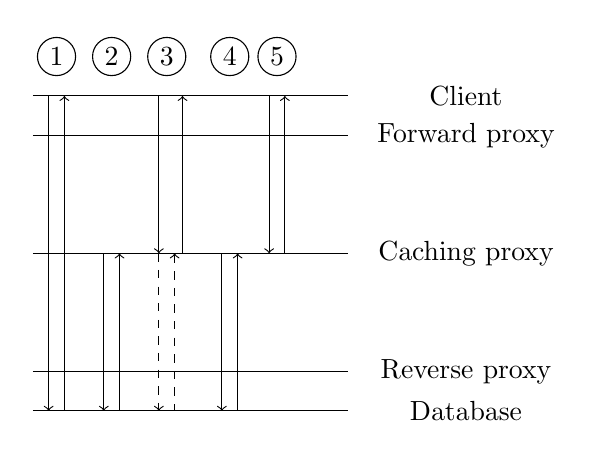
\begin{tikzpicture}
\draw (0,0) --(4,0);
\node at (5.5,0) { Database };
\draw (0,0.5) --(4,0.5);
\node at (5.5,0.5) { Reverse proxy };
\draw (0,2) --(4,2);
\node at (5.5,2) { Caching proxy };
\draw (0,3.5) --(4,3.5);
\node at (5.5,3.5) { Forward proxy };
\draw (0,4) --(4,4);
\node at (5.5,4) { Client };

\draw [->] (0.2,4) --(0.2,0);
\draw [<-] (0.4,4) --(0.4,0);
\node at (0.3,4.5) {\circled{1}};
\draw [->] (0.9,2) --(0.9,0);
\draw [<-] (1.1,2) --(1.1,0);
\node at (1.0,4.5) {\circled{2}};
\draw [->] (1.6,4) --(1.6,2);
\draw [dashed, ->] (1.6,2) --(1.6,0);
\draw [dashed, <-] (1.8,2) --(1.8,0);
\draw [->] (1.9,2) --(1.9,4);
\node at (1.7,4.5) {\circled{3}};
\draw [->] (2.4,2) --(2.4,0);
\draw [<-] (2.6,2) --(2.6,0);
\node at (2.5,4.5) {\circled{4}};
\draw [->] (3,4) --(3,2);
\draw [->] (3.2,2) --(3.2,4);
\node at (3.1,4.5) {\circled{5}};
\end{tikzpicture}
\caption{The possible positions of a cache. A cache may reside at both
  the server side (as a database cache) or client side, or any of the
  intermediate proxies. The arrows illustrate requests (when pointing
  down) and responses (when pointing up) in a deployment scenario for
  when a the query cache considered in this paper is deployed on a
  caching proxy in the Internet infrastructure, see the text for
  details.}\label{fig:messaging}
\end{center}
\end{figure}

The system is based on HTTP, which implies a client-server
architecture. In this architecture, a cache may be present at
conceptually five different levels. First, the client may have its own
cache, which caches only responses made by the client itself. The next
level is known as a forward proxy. They aren't currently very common,
but have in the past often been institutional proxies, or proxies
employed by Internet Service Providers for caching responses that may
be common to many of their users. The next level, generically referred
to as a caching proxy, may be in the Internet
infrastructure. Currently, the most common form of this type of proxy
is known as a Content Delivery Network (CDN). It is very common to
have a reverse proxy near the server. They are often known as a ``Web
Accelerator''. Usually, they will communicate with the server with
HTTP, but it is conceivable that it may use a different protocol, and
may employ detailed knowledge of the hosted data to optimise cache
operations. Finally, the database, in this context a SPARQL Endpoint,
may use conventional database caching techniques. The database cache
and reverse proxy is typically controlled by the data provider.

The present system may be deployed at any of these levels. However,
since the database and the reverse proxy in front of it may have
detailed knowledge of the data, e.g. a complete data profile with
statistics to optimise join order, these levels have much in common
with a conventional database cache, which is extensively discussed in
the literature.

My interest is the case where the caching proxy has no further
knowledge of the data than what is exposed through the SPARQL Endpoint
or hypermedia metadata. In practice, there is very little
information. If the cache is to be shared, then it would typically
reside on the forward proxy, or in a CDN. 

Figure~\ref{fig:messaging} illustrates the case where HTTP messages
are being passed, where the cache is assumed to reside on a
intermediate caching proxy in the Internet, i.e. a CDN. The figure may
be viewed as having time on the $x$-axis, with the arrows pointing
down being requests and the arrows point up being responses. In this
example, the client first makes a request (, which is passed through the
proxy because it has not yet cached any responses. The response is
then also transmitted directly from the SPARQL Endpoint at the
database back to the client. The entire response may be cached at the
proxy in case it can be reused in its entirety. However, 

\bibliography{management,dataprofiles,federation,dynamicity,hypermedia,specs,webarch,practical,semweb,caching,critisism,data,philosophy,benchmarks,rfc,programming,egne}
\bibliographystyle{plain}

\end{document}
